\documentclass[letterpaper, 11pt]{article}

% set version variable
\newcommand{\versionnumber}{0.1}

% russian language
\usepackage[utf8]{inputenc}
\usepackage[T2A]{fontenc}
\usepackage[english, russian]{babel}

% math
\usepackage{mathtools}
\usepackage{amsmath}

\usepackage{amssymb} % some math symbols
% abs function
\DeclarePairedDelimiter{\abs}{\lvert}{\rvert}

% enumerate
\usepackage{enumerate}

% set type and margins of the page
\usepackage{geometry}  % document margins
\geometry{letterpaper, left=1.4in, right = 1.4in, top = 1.7in, bottom = 1.7in}

% color links in content
\usepackage{hyperref}
\hypersetup{
    colorlinks=true,
    linkcolor=red,
    urlcolor=blue,
    linktoc=all
}

% indent at first \par after section
\usepackage{indentfirst}

% fixed table and figures in section
\usepackage{float}

% colors
\usepackage{color}
\usepackage[usenames,dvipsnames]{xcolor}

% paragraph indent
\setlength{\parskip}{0.5em}

% pseudocode
\usepackage{algorithmicx}
\usepackage{algpseudocode}

\title{\large{Краткий конспект}\\
\LARGE{Лекция 5. Преобразование Барроуза-Уилера}\\
\normalsize версия \versionnumber (\textcolor{NavyBlue}{draft})}
\date{28 марта, 2016}
\author{\underline{Д. Ищенко\thanks{МФТИ}} \and Б. Коварский\footnotemark[1]
\and И. Алтухов\footnotemark[1] \and Д. Алексеев\footnotemark[1]}

\begin{document}
\maketitle
\thispagestyle{empty}
\clearpage

% let's go
\section{Оценка памяти необходимой для хранения суффиксного дерева}

На предыдущей лекции мы обсуждали структуру суффиксного дерева и показали, что с помощью него можно решить задачу поиска $k$ мотивов длины $m$ в геноме за $O(km)$. Это очень <<хорошая>> временная сложность и, казалось бы, что можно еще совершенстовать? Зайдем с другой стороны и оценим, какая память необходима для хранения суффиксного дерева? Мы показали, что для последовательности длины $n$, кол-во суффиксов, а значит и листьев в дереве -- $n$ штук. Каждый внутренний узел дерева, в результате ветвления от него, добавляет как минимум один \textit{новый} лист в дерево, т.е. внутренних листов в дереве не больше $n$. Таким образом всего в дереве не больше $2n$ узлов и, соответственно, ребер. Для каждой метки ребра нам нужно хранить 2 числа (начало и конец подпоследовательности в геноме), т.е. для хранения всех меток, нам потребуется $2n \cdot 2 = 4n$ чисел и сам геном длины $n$. В итоге, для хранения всего дерева нам необходимо $2n + 4n + n = 7n$ чисел, а это в семь раз больше, чем требуется для хранения просто последовательности генома.

Например, в случае генома человека длиной $3\cdot10^9$ нуклеотидов, нам было бы необходимо выделить $3Gb \cdot 7 = 21Gb$ оперативной памяти, что, естественно, невозможно сделать на обыкновенном персональном компьютере. Можем ли мы решить эту проблему? Оказывается, что да. Есть несколько вариантов, один из них -- это суффиксные массивы, мы же будем говорить сегодня о \textit{преобразованиях Барроуза-Уилера}. Но прежде, чем перейти непосредственно к преобразованию, разберемся, как мы можем компактно хранить информацию о строках.

\section{Сжатие данных}

Рассмотрим следующую строку длиной 34:
\begin{verbatim}
  AAAAAAAATTTTTTTGGGGGGGAAAAAAAACCCC
\end{verbatim}

Если хранить ее просто, как набор чисел, то нам потребуется 34 байта. Можем ли мы уменьшить это кол-во, не потеряв при этом информации? Можем:

\begin{verbatim}
  8A 7T 7G 8A 4C
\end{verbatim}

Такая краткая запись позволит нам хранить строку, используя всего 10 байт. Важно отметить, что взяв сокращенную запись строки, мы легко можем восстановить исходную. Собственно, этот пример и демонстрирует один из простейших вариантов сжатия данных. Но, что если мы возьмем следующую строку длиной в 8 символов:

\begin{verbatim}
  TATATAGA
\end{verbatim}

Применив вышеописанный подход, мы получим:

\begin{verbatim}
  1T 1A 1T 1A 1T 1A 1G 1A
\end{verbatim}

В рассмотренном случае мы даже увеличили необходимую для хранения строки память. Конечно, мы можем заметить, что в строке идут повторяющиеся блоки TA и записать следующее:

\begin{verbatim}
  3TA 1GA
\end{verbatim}

Но каким образом находить все подобные повторяющиеся блоки? Сколько времени это займет? А как быть, если они идут не подряд? Как работать потом со сжатой таким образом строкой и искать в ней мотивы? Возникает много вопросов и ответом на них и решением задачи сжатия как раз и является преобразование Барроуза-Уилера.

\section{Преобразование Барроуза-Уилера}

Рассмотрим строку S = TATATAGA. Как и при рассмотрении суффиксных деревьев, добавим в конец исследуемой последовательности символ \$. И рассмотрим набор из всех циклических перестановок строки. Он будет иметь следующий вид:
\begin{verbatim}
  T A T A T A G A $
  A T A T A G A $ T
  T A T A G A $ T A
  A T A G A $ T A T
  T A G A $ T A T A
  A G A $ T A T A T
  G A $ T A T A T A
  A $ T A T A T A G
  $ T A T A T A G A
\end{verbatim}

Введем следующее свойтсво алфавита: $\$ < A < C < G < T$. Эта свойство позволяет нам сравнивать между собой символы и производить сортировку строк одинаковой длины. Например две строки ATG и ATA в осортированном порядке:

\begin{verbatim}
ATA
ATG
\end{verbatim}

Первые два символа у них совпадают, а третий $A < G$, поэтому строка ATA идет перед ATG.

Отсортируем все циклические перестановки строки S. Получим следующий набор строк (его можно представить матрицей $M$ размера $n \times n$).

\begin{verbatim}
  F               L
  
  $ T A T A T A G A
  A $ T A T A T A G
  A G A $ T A T A T
  A T A G A $ T A T
  A T A T A G A $ T
  G A $ T A T A T A
  T A G A $ T A T A
  T A T A G A $ T A
  T A T A T A G A $
\end{verbatim}

Назовем первый столбец матрицы -- \textbf{F} (<<first>>) и последний -- \textbf{L} (<<last>>). Очевидно, что первый столбец состоит из подряд идущих блоков состоящих из \$, A, C, G и T, т.к. по нему в первую очередь шла сортировка. Но куда интересней последний столбец \textbf{L} (на самом деле он и представляет из себя преобразование Барроуза-Уилера $BWT(S) = L$). В столбце \textbf{L} тоже встречаются подряд идущие символы, почему так происходит, если сортировка по нему шла в последнюю очередь (после сортировки по всем предыдущим символам)?

Отметим несколько наблюдений: 
\begin{enumerate}[(i)]
\item
символ L[i] \textit{всегда идет перед} символом F[i] в исходной строке S, т.к. каждая строка это циклическая перестановка. 
\item
кажая строка матрицы $M$ начинается с некоторого суффикса строки S, который заканчивается символом \$, т.е. в некотором роде матрица -- это набор всех суффиксов строки S (\textit{аналогия с суффиксным деревом}).
\item
если в строке S, есть повторяющиеся блоки (в нашем случае -- это блоки TA), то строки матрицы, соответствующие суффиксам S, начинающимся с этих блоков идут подряд.
\end{enumerate}

А что, если мы рассмотрим суффиксы (и соответствующие им строки в матрице), которые начинаются со вторых символов повторяющихся блоков? Они тоже должны оказаться рядом в матрице, но при этом первые символы блоков окажутся в последнем столбце матрицы (столбце \textbf{L}) по свойству (i), т.к. они идут перед вторыми символами, а эти символы в повторяющихся блоках одинаковы. Т.е. в \textbf{L} будут стоять подряд идущие одинаковые символы. Чем больше повторяющихся блоков, тем длиннее группы подряд идущих символов в \textbf{L}.

Из этих рассуждений мы и приходим к тому, что при наличии повторов в строке в последнем столбец \textbf{L} находятся группы одинаковых подряд идущих символов. А значит, мы можем <<сжимать>> столбец \textbf{L}, например, описанным ранее способом.

Итак, мы умеем сжимаем столбец \textbf{L}, но пока не знаем самого главного: можем ли мы по столбцу \textbf{L} воостановить исходную строку S? Другими словами, можем ли мы, зная только один столбец \textbf{L}, восстановить всю матрицу M? Оказывается, да. Сделаем еще одно наблюдение:
\begin{enumerate}[(iv)]
\item
в каждом столбце матрицы M представлены все символы из строки S
\end{enumerate}

Чтобы получить первый столбец, достаточно отсортировать все символы столбца \textbf{L}. Используя наблюдение (i), поставим перед столбцом \textbf{F} столбец \textbf{L} и отсортируем такие пары символов, тем самым получим первые два столбца матрицы M. Опять добавим перед осортированными парами столбец \textbf{L} и осортируем тройки символов, получим первые три столбца и т.д. В итоге мы получим всю матрицу M. Для получения исходной строки S, достаточно взять любую строку из матрицы и циклически сдвинуть ее так, чтобы \$ стоял в конце. Готово.

\begin{verbatim}
  L         
 
  A        $      A$        $T      A$T        $TA
  G        A      GA        A$      GA$        A$T
  T        A      TA        AG      TAG        AGA
  T  sort  A  +L  TA  sort  AT  +L  TAT  sort  ATA  etc...
  T   =>   A  =>  TA   =>   AT  =>  TAT   =>   ATA   =>
  A        G      AG        GA      AGA        GA$
  A        T      AT        TA      ATA        TAG
  A        T      AT        TA      ATA        TAT
  $        T      $T        TA      $TA        TAT
\end{verbatim}

Отлично, мы показали возможность восстановления исходной строки из сжатой, хотя и не самым оптимальным способом. Стоит отметить, что этот подход используется, как одна из стадий во многих архиваторах (например, bzip2). Осталось продемонстрировать, как осуществлять поиск мотива в такой строке \textbf{L} (за линейное время) и задача оптимизации памяти будет решена.

Опять же отметим, что результатом преобразования Барроуза-Уилера является столбец \textbf{L}. Т.е. $BWT(S) = L$.

\section{Индексы Ферраджина-Манзини}

В конце XX века Ферраджина и Манзини предложили две функции, названные FM-индексом и позволяющие решить задачу восстановления исходной строки по \textbf{L} и поиска мотива в S за линейное время. Опишем эти две функции.
\begin{enumerate}[I.]
\item
$C(x)$ -- возвращает кол-во символов в строке S, лексиграфически меньших, чем x.
\item
$Occ(x, t)$ -- возвращает кол-во символов x в префиксе строки \textbf{L} длиной $t$ (т.е. в подстроке L[1..t]).
\end{enumerate}

Возвращаемые значения этих функций, удобно представить в виде таблиц. Запишем их для строки S = TATATAGA\$, для которой L = BWT(S) = AGTTTAAA\$.

\begin{table}[H]
\caption{$C(x)$}
\center{
\begin{tabular}{r|ccccc}
  x & \$ & A & C & G & T \\
  \hline
  Occ(x) & 0 & 1 & 5 & 5 & 6 \\
\end{tabular}
}
\end{table}

\begin{table}[H]
\caption{$Occ(x, t)$}
\center{
\begin{tabular}{r|ccccccccc}
  t & 1 & 2 & 3 & 4 & 5 & 6 & 7 & 8 & 9 \\
  L[t] & A & G & T & T & T & A & A & A & \$ \\
  \hline
  \hline
  \$ & 0 & 0 & 0 & 0 & 0 & 0 & 0 & 0 & 1 \\ 
  A  & 1 & 1 & 1 & 1 & 1 & 2 & 3 & 4 & 4 \\
  C  & 0 & 0 & 0 & 0 & 0 & 0 & 0 & 0 & 0 \\
  G  & 0 & 1 & 1 & 1 & 1 & 1 & 1 & 1 & 1 \\
  T  & 0 & 0 & 1 & 2 & 3 & 3 & 3 & 3 & 3 \\
\end{tabular}
}
\end{table}

Что позволяют делать эти две функции? Пусть $i$-ый символ в столбце \textbf{L} это $j$-ый символ в строке S (L[i] = S[j]), с помощью функций $C(X)$ и $Occ(x)$ мы можем определить позицию этого же символа (S[j]) в столбце \textbf{F}. 

Прежде, чем показать, как это сделать, докажем один интересный факт. Проставим каждому символу в \textbf{F} ранг, другими словами его порядковый номер среди всех идентичных ему символов, двигаясь сверху-вниз (красные цифры на Рис. 1). Тем самым мы каждому символу присвоим уникальный номер среди всех ему подобных. Отметим эти же номера в последнем столбце \textbf{L}, здесь подразумевается не новое проставление рангов, а сохранение рангов из первого столбца, например, $A_1$ из \textbf{F} это восьмой символ в строке S, этот же символ находится первым в \textbf{L}, значит его ранг тоже $A_1$. Так вот: \textit{последовательность рангов в последнем столбце не будет нарушена}. Т.е. второй сверху нуклеотид <<A>> в первом столбце также будет вторым сверху в последнем.
\begin{figure}[H]
  \center{
  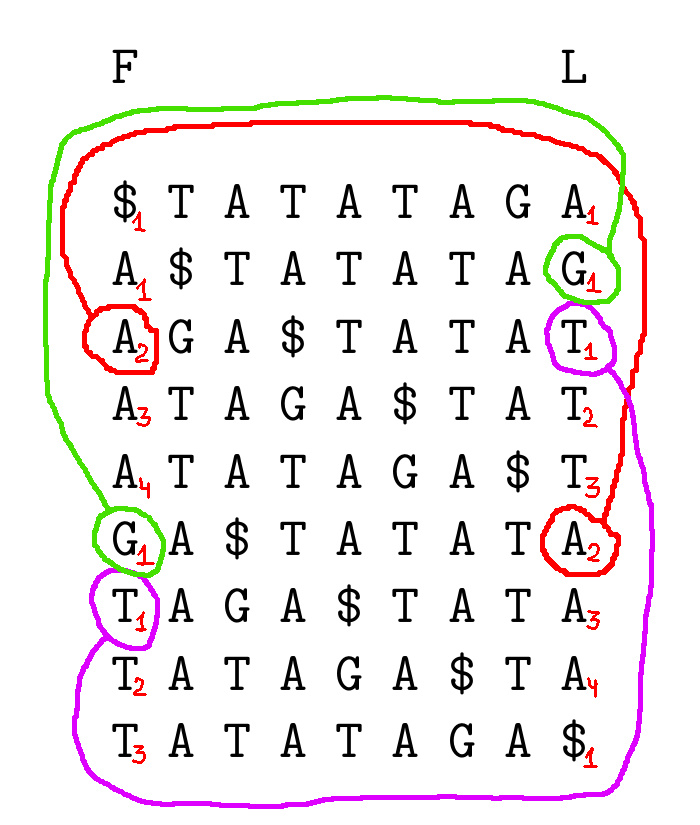
\includegraphics[scale=.3]{fig/ranks.jpg}
  }
  \caption{Пример сохранения рангов в \textbf{F} и \textbf{L}.}
\end{figure}

Откуда это следует? Рассмотрим, например, все строки в M, начинающиеся на T (в \textbf{F} стоит T), пусть они составляют множество {$\Psi$}, очевидно, что они идут подряд и отсортированы. Строки, которые заканчиваются на T (у которых в \textbf{L} стоит T), образованы из всех строк $\Psi$ циклическим сдвигом на одну позицию <<влево>>. Причем, находятся они в матрице в отсортированном порядке, начиная с их первого символа (второго относительно $\Psi$). Но в множестве $\Psi$ они были точно в таком же порядке, т.к. первый символ у всех строк из $\Psi$ одинаковый (равен T), значит они сортировались по второму, третьему и т.д. символам.

Что это дает? Зная ранг $i$-го символа в последнем столбце $rank(x)$, мы легко можем определить его позицию в первом столбце. Этот переход задается функцией <<last-to-first>>:

$$LF(i) = C(L[i]) + rank(L[i])$$

Заметим, что $rank(L[i]) = Occ(L[i], i)$, т.к. как ранг -- это и есть количество вхождений символа в префикс, тогда:

$$LF(i) = C(L[i]) + Occ(L[i], i)$$

Для $i$-го символа в столбце \textbf{F} мы можем определить символ, который идет перед ним в строке S, просто посмотрев в этой же строке символ L[i]. Для L[i] с помощью функции $LF(i)$ мы можем определить строку, в которой L[i] стоит в первым в строке, пусть это строка $j = LF(i)$. Теперь мы можем узнать, что идет в S перед этим символом опять же посмотрев последний символ в $j$, т.е. L[j] и т.д. Т.е. такими циклическими переходами мы можем восстановить всю строку.

\section{Поиск мотива}
Эта же логика применяется при поиске мотива в строке. Допустим, мы хотим определить кол-во вхождений мотива TAT в строку S. Будем двигаться \textit{от последнего символа мотива к первому}, начинаем с символа T, находим строки, которые начинаются с T, это строки с индексами $\{8, 9, 10\}$ (мы легко это можем сделать с помощью $C(x)$, Рис. 2). Следующий символ с конца в мотиве -- A, в отобранных нами строках перед символами T, идут символы, которые находятся в последнем столбце в $\{8, 9, 10\}$ строках, выберем из них те, которые оканчиваются на A, это строки $\{8, 9\}$ с $A_3$ и $A_4$ в конце. Найдем строки, которые начинаются с $A_3$ и $A_4$ -- это $\{4, 5\}$ строки (этот переход мы легко сможем совершить с помощью функции $LF(i)$). Берем следующий символ мотива с конца -- T. Находим в отобранных нами строках, заканчивающиеся на T, они обе подходят и заканчиваются на $T_2$ и $T_3$, перейдем к строкам (с помощью $LF(i)$), начинающимися на эти T -- это строки $\{8, 9\}$. Собственно все, мы прошли по всем символам мотива и определили строки, а значит суффиксы и кол-во вхождений мотива в геном S.

\begin{figure}[H]
  \center{
  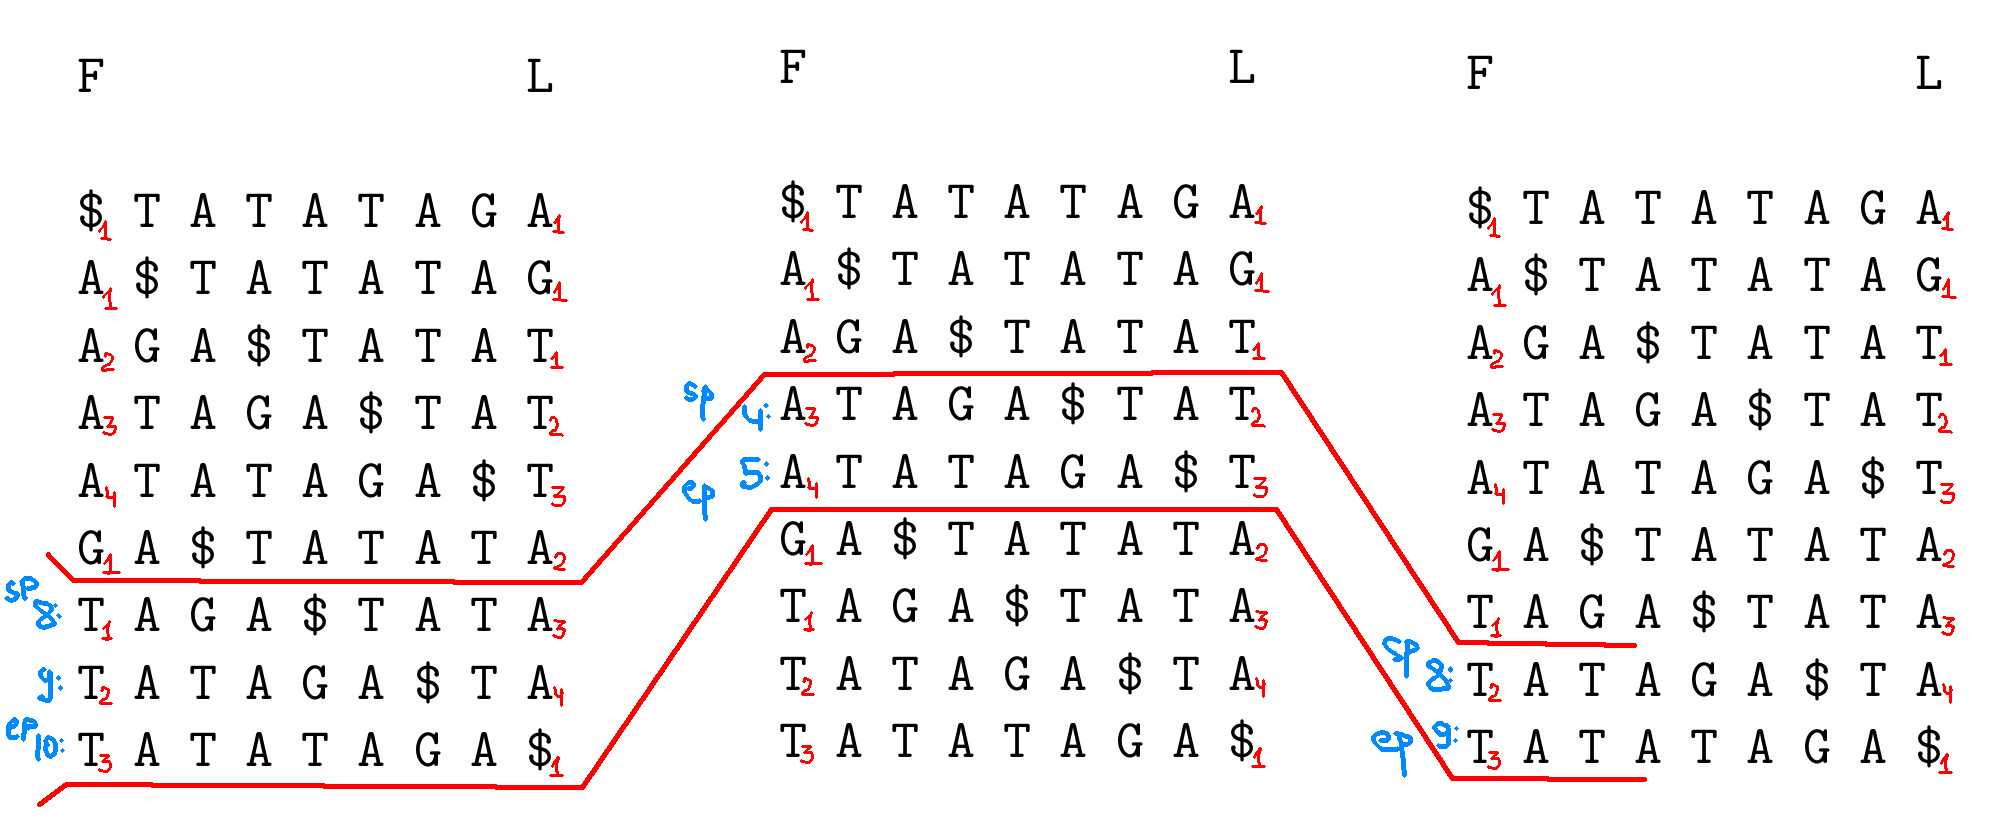
\includegraphics[scale=0.2]{fig/motif.jpg}
  }
  \caption{Поиск мотива TAT с помощью преобразования Бароуза-Уилера и индексов Ферраджина-Манзини}
\end{figure}

\section{Как хранить $C(x)$ и $Occ(x, t)$?}
\section{Ссылки}

\begingroup
\renewcommand{\section}[2]{}%
\begin{thebibliography}{7}
\bibitem{BW}
Burrows M., Wheeler D. A block-sorting lossless data compression algorithm //DIGITAL SRC RESEARCH REPORT. – 1994.
\bibitem{FM}
Ferragina P., Manzini G. Opportunistic data structures with applications //Foundations of Computer Science, 2000. Proceedings. 41st Annual Symposium on. – IEEE, 2000. – С. 390-398.

\end{thebibliography}
\endgroup

\end{document}
